In this section, we formally introduce the minimal-information control of MDPs.
After we describe a general framework in Section~\ref{secformulation}, we discuss how the framework can incorporate the problem of synthesizing a minimal-information policy under temporal logic constraints.

\subsection{Mathematical formulation}
\label{secformulation}

Let $M=(\mathcal{X}, \mathcal{U}, p)$ be a finite MDP with state-action cost $c_t(x_t, u_t, x_{t+1})$. Let $q_t(u_t|x^t,u^{t-1})$ be the policy to be synthesized. The expected accumulated cost over a time horizon $0\leq t \leq T-1$ is denoted by
\[
J(X^T, U^{T-1})=\sum_{t=0}^{T-1}\mathbb{E}\{c_t(x_t, u_t, x_{t+1})\}.
\]
Suppose that the state space of $M$ is split into the space $\bar{\mathcal{X}}$ of ``expensive to observe'' state variables and the space $\tilde{\mathcal{X}}$ of ``free'' state variables as $\mathcal{X}=\bar{\mathcal{X}}\times \tilde{\mathcal{X}}$.
At every time step, observing a realization of the ``free'' component $\tilde{X}_t$ of the state random variable $X_t=(\bar{X}_t, \tilde{X}_t)$ is free of charge, whereas observing the ``expensive'' component $\bar{X}_t$ incurs cost. 

As an example, imagine the MDP models a Mars rover. The value of $\bar{x}$ is measured by an orbiter or a scouting helicopter while $\tilde{x}$ is sensed using on-board sensors. Since the orbiter will only be able to communicate with the rover during part of its orbit, we will want to penalize the reliance on this information in the policy synthesis process. In the case of the helicopter we want to limit the transmission between them as this can consume a lot of power. We can represent this as a feedback control architecture shown in Figure~\ref{fig:NCS}. 
\begin{figure}
\centering
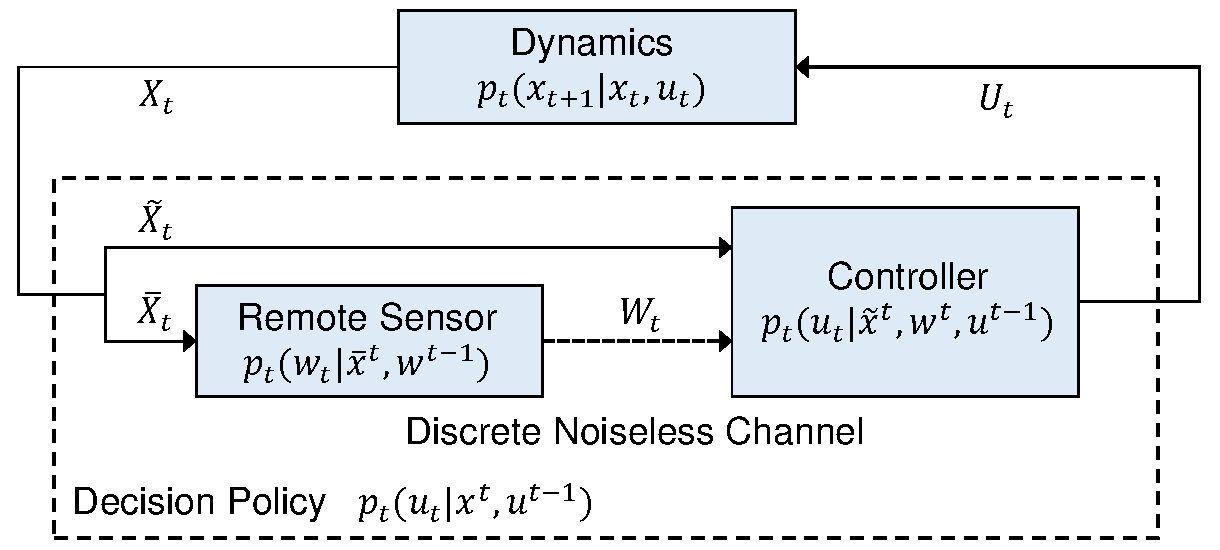
\includegraphics[width=\columnwidth]{comm.pdf}
\caption{Example of a feedback control structure with remote and local sensors}
\label{fig:NCS}
\end{figure}

At every time step $t$, assume that the free component $\tilde{X}_t$ of the state vector is immediately available to the rover, i.e, from onboard sensors, while the expensive component $\bar{X}_t$ is only available from a remote sensor, i.e, the scouting helicopter. Before the state information can be transmitted, the remote sensor has to encode it into bits. The remote sensor produces a discrete codeword $W_t\in\mathcal{W}_t$ representing the state information based on a policy $p_t(w_t|\bar{x}^t, w^{t-1})$, where $\mathcal{W}_t$ is a certain codebook such that $|\mathcal{W}_t|=2^{R_t}$. The codeword is transmitted over a noiseless communication channel and received by the controller without delay, and a control input $U_t$ is generated based on a policy $p_t(u_t|\tilde{x}^t, w^t, u^{t-1})$. We aim to limiting the data transfer from the remote sensor to on-board controller. 

 We now introduce some information-theoretic terms. 

The \emph{joint distribution} $\mu_{t}(x^{t}, u^{t-1})$ defined recursively by the state transition probability $p_t(x_{t+1}|x_t, u_t)$ and a decision policy $q_t(u_t|x^t, u^{t-1})$ as
\[
\mu_{t+1}(x^{t+1}, u^t)=p_t(x_{t+1}|x_t, u_t)q_t(u_t|x^t, u^{t-1})\mu_t(x^t, u^{t-1}).
\]


 The \emph{conditional mutual information} is given by 

\begin{align*}
I  (\bar{X}^t;U_t & \vert U^{t-1},\tilde{X}^{t}) \defeq \nonumber \\ &\mathbb{E}_{\mu_T}\bigg\{\log\frac{\mu_{t}(U_t|\bar{X}^{t},U^{t-1},\tilde{X}^t)}{\mu_{t}(U_t\vert U^{t-1}, \tilde{X})^t}\bigg\}.
\end{align*}

We assume that the observation cost over the time horizon $0\leq t\leq T-1$ is proportional to the \emph{causally conditioned directed information} (also known as \emph{causally conditioned transfer entropy}).
\begin{equation}
\label{eqdi}
I(\bar{X}^{T-1}\rightarrow U^{T-1}\| \tilde{X}^{T-1})=\sum_{t=0}^{T-1} I(\bar{X}^t; U_t|U^{t-1},\tilde{X}^t).
\end{equation}
We note that the notion of \emph{directed information} is introduced by \cite{massey1990causality} based on \cite{marko1973bidirectional}, and its generalization with causal conditioning by \cite{kramer1998causal}. Intuitively, \eqref{eqdi} can be understood as the information flow from a random process $\{\bar{X}_t\}$ to $\{U_t\}$ given $\{\tilde{X}_t\}$ as side information.
The main problem we study in this paper is
\begin{align}
\min_{\{q_t(u_t|x^t,u^{t-1})\}_{t=0}^{T-1}} & J(X^T, U^{T-1}) \nonumber \\
&+\beta I(\bar{X}^{T-1}\rightarrow U^{T-1}\| \tilde{X}^{T-1}) \label{eqmainproblem}
\end{align}
where $\beta>0$ is a given constant.


Assuming that transmitting data over the communication channel incurs unit cost $\beta$ per \emph{bit}, consider the following communication design problem
\begin{equation}
\min_{\{\mathcal{W}_t, p_t(w_t|\bar{x}^t, w^{t-1}), p_t(u_t|\tilde{x}^t, w^t, u^{t-1}) \}_{t=0}^{T-1}}  J(X^T, U^{T-1}) +\beta R \label{eqcommproblem}
\end{equation}
where $R=\sum_{t=0}^{T-1}R_t$ is the total amount of data. 
The next result shows that \eqref{eqdi} provides a lower bound to $R$.
\begin{theorem}
\label{theorate}
Suppose that the plant dynamics is given by an MDP $M$. For any choice of the codebook $\mathcal{W}_t$, sensor policy $p_t(w_t|\bar{x}^t, w^{t-1})$ and controller policy $p_t(u_t|\tilde{x}^t, w^t, u^{t-1})$ for $0\leq t\leq T-1$ in Figure~\ref{fig:NCS}, we have
\[
R \geq I(\bar{X}^{T-1}\rightarrow U^{T-1}\| \tilde{X}^{T-1}).
\]
\end{theorem}
\begin{proof}
See Appendix \ref{sec:prf}
\end{proof}
Theorem~\ref{theorate} shows that the optimization problem \eqref{eqmainproblem} provides a fundamental performance limitation of the networked control system shown in Figure~\ref{fig:NCS} in that the optimal value of \eqref{eqcommproblem} is lower bounded by the optimal value of \eqref{eqmainproblem}.
%
%
%A communication-theoretic meaning of the optimization problem \eqref{eqmainproblem} is discussed in section \ref{sec:ab} where we provide a physical interpretation of the transfer entropy cost.

% can be given by considering a feedback control architecture shown in Figure \ref{fig:NCS}. 
%At every time step $t$, assume that the free component $\tilde{X}_t$ of the state vector is immediately available to the controller, while the expensive component $\bar{X}_t$ is only available at a remote sensor. The remote sensor produces a discrete codeword $W_t\in\mathcal{W}_t$ based on a policy $p_t(w_t|\bar{x}^t, w^{t-1})$, where $\mathcal{W}_t$ is a certain codebook such that $|\mathcal{W}_t|=2^{R_t}$. Codeword is transmitted over a noiseless communication channel and received by the controller without delay, and a control input $U_t$ is generated based on a policy $p_t(u_t|\tilde{x}^t, w^t, u^{t-1})$. The transfer entropy cost in \eqref{eqdi} can be used to model the \emph{communication rate}. In section \ref{sec:ab}, we present a formal proof showing that \eqref{eqdi} provides a lower bound to the communication rate to justify its use in our problem formulation.

%Consider the control system architecture shown in Figure \ref{fig:NCS} modeled by a finite state discrete-time MDP. The state space $\mathcal{X}$ is composed of the product of two sets  $\mathcal{X} = \mathcal{X}_e \times \mathcal{X}_f$. Hence, each state in the state space $x \in \mathcal{X}$ is partitioned into two state variables $x = (x_e,x_f)$. Recall that a policy is a conditional policy distribution given by $q(u_t|x^t,u^{t-1})$. We can write this now as $q(u_t|x_e^t,x_f^t,u^{t-1})$. We allow the policy synthesizer full access to the value of $x_f$, but we restrict access to the value of $x_e$. 



%Let $\tilde{X} \in \mathcal{\tilde{X}}$, $\overline{X} \in \mathcal{\overline{X}}$, $U\in \mathcal{U}$ be random variables of which $\tilde{x},\overline{x},u$ are realizations. The \emph{conditional mutual information} is 
%
%\begin{align*}
%I  (X_{e_{t-m}}^t;U_t & \vert U^{t-1}_{t-n},X_{f_{t-m}}^{t}) \defeq \nonumber \\ &\sum_{\mathcal{X}^{t}_f}\sum_{\mathcal{U}^{t-1}}\log\frac{\mu_{t+1}(u_t|x_{t-m}^{t},u_{t-n}^{t-1})}{\mu_{t+1}(u_t\vert u_{t-n}^{t-1})}
%\end{align*}\todo{Fix definition}



%The transfer entropy of degree $(m,n)$ is defined as \cite{schreiber2000}
%
%\begin{align}\label{eqn:TEcond}
%I_{m,n}(X_e^T  \rightarrow & U^{T-1}||X_f^T) \defeq \nonumber \\ & \sum_{t=0}^{T-1} I\left(X_{e_{t-m}}^t;U_t|U^{t-1}_{t-n},X_{f_{t-m}}^{t} \right) .
%\end{align}
%




% An \emph{encoder} and \emph{decoder} are defined as stochastic kernels $e_t(w_t|x^t,w^{t-1})$ and $d_t(u_t|w^t,u^{t-1})$ respectively. $w_t$ is a \emph{codeword} chosen from \emph{codebook} $\mathcal{W}_t$ at time $t$. $|\mathcal{W}_t| = 2^{R_t}$. $R = \sum_{t=1}^T$ is the rate of communication. 

% For example in Figure \ref{fig:NCS}, at each time step the sensor sends data to the encoder which chooses a codeword $w_t$ and passes the message to the decoder. 


% \paragraph{Optimal policy}
% Given an MDP $M=(\mathcal{X},\mathcal{U},p)$ with cost function $c_t: \mathcal{X} \times \mathcal{U} \rightarrow \mathbb{R}$, and finite time horizon $T$, the optimal policy $q$ is one that minimizes the following

% \begin{equation}\label{eqn:optpol}
% J(X^T,U^{T-1}) \defeq \sum_{t=0}^{T-1}{\mathbb{E}\{c_t(X_t,U_t)\}} + \mathbb{E}\{c_{T}(X_{T})\}
% \end{equation}

% Informally, the policy minimizes the expected value of the cost over the time horizon. In this setting the optimal policy will be deterministic and Markovian. 

% \paragraph{Expensive-to-measure state variable} We divide the state space $\mathcal{X}$ into expensive and free to measure state variables, \ie $\mathcal{X} = \mathcal{X}_e \times \mathcal{X}_f$. A state $x \in \mathcal{X}$ can be expressed as $x = (x_e,x_f)$ where $x_e \in \mathcal{X}_e$ is expensive-to-measure and $x_f \in \mathcal{X}_f$ is free. 

% Now, consider the following information-constrained optimal control problem:
% \begin{equation}
% \min_{\{q_t\}_{t=1}^T} J(X^{T},U^{T-1}) + \beta \sum_{t=0}^T R_t
% \end{equation}
% where $\beta \in \mathbb{R}$, $R = \sum_{t=0}^T R_t$ is the rate of communication, and $J(X^T,U^{T-1}) \defeq \sum_{t=0}^{T-1}{\mathbb{E}\{c(X_t,U_t)\}} + \mathbb{E}\{c_{T}(X_{T})\}$ for some state-action dependent cost $c(X_t,U_t) \in \mathbb{R}$. 

%\begin{figure}
%\centering
%\begin{tikzpicture}[auto, node distance=2cm,>=latex']
%    % We start by placing the blocks
%    \node [input, name=input] {};
%    \node [sum, right of=input] (sum) {};
%    \node [block, right of=sum,text width=2.1cm] (controller) {\textbf{Controller}\\$q_t(u_t|x^t,u^{t-1})$};
%    \node [block, right of=controller,node distance = 3cm,text width=2cm] (dynamics) {\textbf{Dynamics}\\$p(x_{t+1}|x_t,u_t)$};
%    % We draw an edge between the controller and system block to 
%    % calculate the coordinate u. We need it to place the measurement block. 
%    \node [output, right of=dynamics] (output) {};
%    \node [sblock, below of=dynamics,text width = 1cm] (xc) {\textbf{Sensor}\\ \textit{Costly}};
%    \node [sblock, left of=xc] (encoder) {\textbf{Encoder}};
%	\node [sblock, below of=xc,node distance = 1.5cm, text width = 1cm] (xf) {\textbf{Sensor}\\\textit{Free}};
%	\node [sblock, left of=encoder,node distance = 2cm] (decoder) {\textbf{Decoder}};
%    % Once the nodes are placed, connecting them is easy. 
%    \draw [draw,->] (input) -- node {} (sum);
%    \draw [->] (sum) -- node {$X_t$} (controller);
%    \draw [->] (controller) -- node {$u_t$} (dynamics);
%    \draw [->] (dynamics) -- node [name=y] {$X_{t+1}$}(output);
%    \draw [->] (y) |- (xc);
%    \draw [->] (xc) -- node {$\bar{X}_t$} (encoder);
%    \draw [->] (y) |-  (xf);
%    \draw [->] (encoder) -- node {$W$} (decoder);
%     \draw [->] (decoder) -| node {$(\bar{X}_t,\tilde{X}_t)$} (sum);
%    \draw [->] (xf) -| node {$\tilde{X}_t$}(sum);
%\end{tikzpicture}\caption{Control system architecture where $\bar{X}_t$ is sensed remotely and has to be transmitted to the controller through an encoder-decoder system.}\label{fig:NCS}
%
%\end{figure}


